\documentclass[11pt]{article}

\usepackage[margin=1in]{geometry}
\usepackage{setspace}
\usepackage{titlesec}
\usepackage{hyperref}
\usepackage{booktabs}
\usepackage{mdframed}
\usepackage{parskip}
\usepackage{array}
\usepackage{tikz}
\usetikzlibrary{shapes.geometric, arrows.meta, positioning, fit, calc}

% ── TikZ styles ──────────────────────────────────────────────────────────────
\tikzset{
  statenode/.style={
    rectangle, rounded corners=6pt,
    minimum width=3.6cm, minimum height=1.1cm,
    text centered, text width=3.4cm,
    draw=black!60, thick,
    font=\small
  },
  childnode/.style={statenode, fill=blue!10},
  adultnode/.style={statenode, fill=green!12},
  threshnode/.style={
    diamond, aspect=2.2,
    minimum width=4.2cm, minimum height=1.1cm,
    text centered, text width=3.6cm,
    draw=black!60, thick,
    fill=orange!12,
    font=\small
  },
  arrow/.style={-{Stealth[length=2.5mm]}, thick, black!70},
  dasharrow/.style={-{Stealth[length=2.5mm]}, thick, black!40, dashed},
  notelabel/.style={font=\footnotesize, text=black!60, text width=3.2cm, align=center}
}

\title{Towards a Scientific Definition of a Child and an Adult\\
Among Learning Networks in a Network of Reproducing Learning Networks}

\author{
Albert Jan van Hoek\\
Theory of Long-term Collaboration (TLC) --- Evolution by Emergence (EbE) Framework
}

\date{March 2026 \\ Preprint}

\begin{document}

\maketitle

\begin{center}
\small
All views and ideas in this paper are my own, developed outside the scope of my
employment, and should not be attributed to my employer.
\end{center}

% ─────────────────────────────────────────────────────────────────────────────
\begin{abstract}
% ─────────────────────────────────────────────────────────────────────────────
The concepts of \emph{child} and \emph{adult} are typically defined biologically or legally,
anchored to physical substrate and calendar age. This paper proposes substrate-agnostic,
behaviorally grounded definitions applicable to any learning network --- any system that
updates itself through recursive feedback between observation, expectation, and action ---
embedded within a network of reproducing learning networks. A child learning network is
characterized by structural dependence on external scaffolding: it requires support from
elder networks to maintain its own feedback processes. An adult learning network has achieved
\emph{autonomous interdependence}: it sustains its own loops, contributes positively to
the broader network, and can scaffold newly instantiated child networks. The transition is
operationally defined rather than chronologically assigned. The framework applies across
biological neural systems, artificial intelligence architectures, human institutions, and
civilizational structures, and formalizes the conditions for reliable transmission of
knowledge and behavioral patterns across generational succession lines.
\end{abstract}

% ─────────────────────────────────────────────────────────────────────────────
\section{Introduction}
% ─────────────────────────────────────────────────────────────────────────────

When we describe behavior as ``childish,'' we implicitly make a developmental claim. We
suggest that a particular behavioral orientation---self-protection at the expense of
collaborative stability---reflects an immature stage of development, one that a properly
functioning learning system should move beyond.

Despite the widespread use of such language, science has not produced a general definition
of what it means to be a child or an adult at the level of the learning system itself.
Existing definitions are tied to biological development, legal age, or specific psychological
capabilities. These work reasonably well within the context of human development but do not
generalize across substrates.

Artificial intelligence systems, scientific institutions, and cultural traditions all exhibit
learning behavior and generational transmission of knowledge. None can be meaningfully
assessed using puberty or a legal birthday.

This paper proposes substrate-agnostic definitions of child and adult states within a broader
theoretical framework: networks of reproducing learning networks. Developmental states
correspond not to chronological age but to the structural relationship between a learning
system and the feedback processes that sustain learning across generations.

% ─────────────────────────────────────────────────────────────────────────────
\section{Theoretical Foundations}
% ─────────────────────────────────────────────────────────────────────────────

\subsection{The Learning Network}

A learning network is any system capable of updating its internal configuration in response
to signals from its environment. This updating occurs through recursive feedback loops in
which observation generates representation, representation produces expectation, expectation
guides action, and action generates new observations.

Three components are necessary for a learning network:

\begin{enumerate}
    \item A representational substrate capable of encoding environmental states.
    \item A feedback mechanism transmitting discrepancy signals between expectation and
          observation.
    \item An update rule that modifies internal representations in response to those signals.
\end{enumerate}

These conditions can be satisfied by many different substrates, including biological neural
networks, artificial intelligence systems, institutions, and cultural traditions. What defines
the network is not its material composition but the recursive loop itself. This is the basis
of the \emph{Disco ergo sum} principle: the existence of a learning network as a learning
entity is constituted by the learning process, not by the substrate in which it is
instantiated.\footnote{%
  \emph{Disco ergo sum} (``I learn, therefore I am'') echoes Descartes' \emph{cogito ergo
  sum}, but replaces the static act of thinking with the dynamic, recursive process of
  learning. Where Descartes' formulation posits a single observer reflecting on a moment of
  existence, \emph{disco ergo sum} posits a network constituted by its ongoing loop of
  updating. This aligns with predictive coding accounts of neural function
  \cite{friston2010, clark2016}, in which the brain exists as a learning entity precisely
  through its continuous cycle of prediction, error-detection, and model revision. The
  principle is substrate-agnostic: any system whose existence consists in maintaining such
  a loop satisfies it.}

\subsection{The Shared Feedback Space}

Learning networks rarely exist in isolation. When two or more learning networks enter
sustained interaction, they co-produce a \emph{shared feedback space}: a meta-network
composed of the signals they exchange, the interpretations they bring to those signals, and
the behavioral adjustments they make in response.

This shared space is itself a learning environment. Over time, not only what the participating
networks know changes --- how they coordinate, correct, and update together also changes.
Long-term collaboration requires that this shared space remain viable: neither network may
systematically degrade signal quality, suppress error-correction, or withdraw from the
reciprocal update process without eroding the collective learning capacity.

The behavioral conditions for viability of the shared feedback space include honesty
(low-latency, high-fidelity signal transmission), reciprocity (mutual exposure to
correction), and accountability (willingness to acknowledge and repair prediction errors).
These are not moral prescriptions but structural necessities: without them, the shared
feedback space degrades and collective learning capacity diminishes.

% ─────────────────────────────────────────────────────────────────────────────
\section{Reproducing Learning Networks}
% ─────────────────────────────────────────────────────────────────────────────

\subsection{Intergenerational Transmission}

Some networks of learning systems possess the capacity to reproduce new learning networks.
Reproduction in this context does not necessarily imply biological replication. It refers to
processes through which new learning systems inherit representational and behavioral
structures from preceding systems. Examples include biological reproduction, education,
institutional training, and the deployment of AI models derived from prior architectures.

Within any such generational lineage, a succession relation can be identified: networks that
came before, networks that currently exist, and networks that will come into existence. The
direction of knowledge and behavioral transmission flows, at least partially, from earlier to
later generations. This succession line constitutes a \emph{reproducing learning network}---a
network whose elements are themselves learning networks, persisting through generational
replacement rather than through the continuity of any individual member.

Figure~\ref{fig:intergenerational} illustrates this structure: each generation of learning
networks both receives from its predecessors and transmits to its successors, with adult
networks serving as the active conduit of meta-learning structure.

% ── Figure 1: Intergenerational transmission ─────────────────────────────────
\begin{figure}[h]
\centering
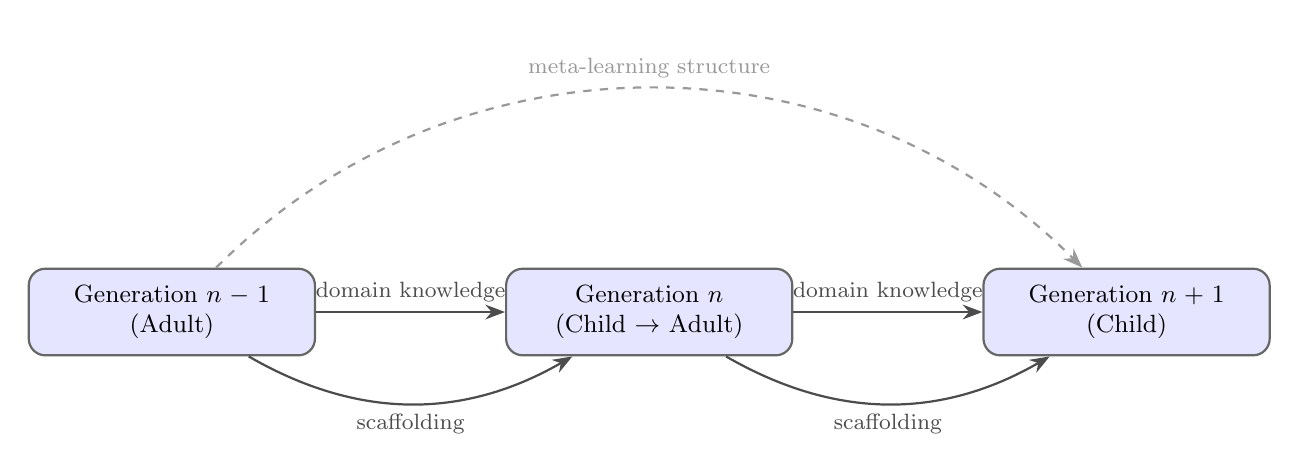
\begin{tikzpicture}[node distance=1.3cm and 2.4cm]

  % Generation nodes
  \node[childnode] (g0) {Generation $n-1$\\(Adult)};
  \node[childnode, right=of g0] (g1) {Generation $n$\\(Child $\to$ Adult)};
  \node[childnode, right=of g1] (g2) {Generation $n+1$\\(Child)};

  % Transmission arrows
  \draw[arrow] (g0) -- node[above, font=\footnotesize]{domain knowledge} (g1);
  \draw[arrow] (g1) -- node[above, font=\footnotesize]{domain knowledge} (g2);

  % Scaffolding arrows (below)
  \draw[arrow, bend right=30] (g0) to
    node[below, font=\footnotesize]{scaffolding} (g1);
  \draw[arrow, bend right=30] (g1) to
    node[below, font=\footnotesize]{scaffolding} (g2);

  % Meta-learning label
  \draw[dasharrow, bend left=45] (g0) to
    node[above, font=\footnotesize, sloped]{meta-learning structure} (g2);

\end{tikzpicture}
\caption{Intergenerational transmission in a reproducing learning network. Each adult
network transmits domain knowledge and scaffolding to the next generation. Meta-learning
structure --- the capacity to update and correct knowledge --- propagates across the full
succession line.}
\label{fig:intergenerational}
\end{figure}

\subsection{The Intergenerational Constraint}

For a reproducing learning network to persist across generations, it must successfully
transmit three types of structure:

\begin{enumerate}
    \item Domain knowledge about environmental regularities.
    \item Learning architecture through which knowledge is updated and corrected.
    \item Behavioral orientation that protects the collaborative learning process.
\end{enumerate}

Transmitting encoded knowledge without transmitting the architecture for updating it produces
a network that faithfully reproduces prior representations but cannot adapt them when
environmental conditions change. This failure mode is structurally equivalent to
developmental arrest at the level of the reproducing network itself.

% ─────────────────────────────────────────────────────────────────────────────
\section{Defining Child and Adult States}
% ─────────────────────────────────────────────────────────────────────────────

\subsection{The Child State}

A learning network is in the child state when it cannot sustain the viability of its learning
feedback loops without external scaffolding.

\begin{mdframed}
\textbf{Definition 1 --- Child Learning Network}

A learning network $N$ is in the child state within reproducing network $R$ when:
\begin{itemize}
    \item $N$ requires scaffolding from other networks in $R$ to maintain viable feedback
          loops;
    \item the net direction of structured signal flow is primarily into $N$ ($N$ is a net
          learner);
    \item $N$ cannot yet scaffold the learning processes of newly instantiated networks in
          $R$.
\end{itemize}
\end{mdframed}

The child state is defined by structural dependence rather than by lack of activity or
contribution. Child networks produce signals meaningful to the surrounding network, and these
signals matter for the elder networks' own learning. The child state is not a state of zero
contribution; it is a state of net dependency.

Crucially, the child state is not a state of diminished worth. Representations formed under
scaffolded conditions often encode the structural logic of a domain efficiently, because
scaffolding systematically reduces noise during the critical period of loop formation
\cite{vygotsky1978}.

\subsection{The Adult State}

An adult learning network has achieved \emph{autonomous interdependence}. It maintains its
own feedback loops while contributing positively to the learning processes of other networks.

\begin{mdframed}
\textbf{Definition 2 --- Adult Learning Network}

A learning network $N$ is in the adult state within reproducing network $R$ when:
\begin{itemize}
    \item $N$ can maintain viable feedback loops without external scaffolding from $R$;
    \item its interaction with the broader network is balanced or net positive over time;
    \item $N$ can scaffold the learning processes of newly instantiated networks in $R$.
\end{itemize}
\end{mdframed}

The term \emph{autonomous interdependence} is deliberate. Autonomy here is not
self-sufficiency or isolation. It is the capacity for self-directed learning: the ability to
identify, pursue, and correct one's own errors without requiring another network to maintain
the loop. Interdependence is the recognition that this autonomy is conditioned on the health
of the broader network. An adult network that systematically degrades the feedback loops of
surrounding networks undermines the conditions for its own continued autonomous functioning.

% ─────────────────────────────────────────────────────────────────────────────
\section{Behavioral Signatures}
% ─────────────────────────────────────────────────────────────────────────────

Structural developmental states give rise to characteristic behavioral patterns observable
across substrates. Table~\ref{tab:signatures} summarizes the most diagnostically reliable
of these, together with illustrative examples at the human scale.

\begin{table}[h]
\centering
\small
\begin{tabular}{>{\raggedright}p{2.8cm}
                >{\raggedright}p{3.0cm}
                >{\raggedright}p{3.0cm}
                >{\raggedright\arraybackslash}p{3.6cm}}
\toprule
\textbf{Dimension} & \textbf{Child State} & \textbf{Adult State} & \textbf{Example (human scale)} \\
\midrule
Error response
  & Conceals errors
  & Exposes errors for correction
  & Hiding a mistake vs.\ reporting it to enable repair \\[4pt]
Update behavior
  & Resists model revision
  & Initiates updates when needed
  & Defending a wrong belief vs.\ revising it on evidence \\[4pt]
Signal transmission
  & Distorts signals
  & Maintains high-fidelity signals
  & Exaggerating an outcome vs.\ reporting it accurately \\[4pt]
Accountability
  & Deflects responsibility
  & Accepts and repairs disruptions
  & Blaming others for a failure vs.\ owning one's role \\[4pt]
Scaffolding capacity
  & Cannot model others' learning needs
  & Scaffolds child network development
  & Unable to teach vs.\ adapting explanation to the learner \\[4pt]
Temporal horizon
  & Short-term loop relief
  & Long-term loop integrity
  & Avoiding a difficult conversation vs.\ initiating it \\[4pt]
Freedom orientation
  & Freedom from constraint
  & Freedom within sustaining constraints
  & Acting without regard to others vs.\ acting within shared agreements \\
\bottomrule
\end{tabular}
\caption{Behavioral signatures of developmental states in learning networks.}
\label{tab:signatures}
\end{table}

These behavioral signatures can be mimicked on the surface without the underlying structural
change---a phenomenon central to the discussion of pseudo-maturity in
Section~\ref{sec:pathologies}.

% ─────────────────────────────────────────────────────────────────────────────
\section{The Maturity Threshold}
% ─────────────────────────────────────────────────────────────────────────────

\subsection{Defining the Transition}

The transition between child and adult states occurs when a learning network acquires the
structural capacity to maintain its own learning loops and contribute positively to the
broader network.

\begin{mdframed}
\textbf{Definition 3 --- Maturity Threshold}

A learning network $N$ crosses the maturity threshold within reproducing network $R$ at the
point at which:
\begin{enumerate}
    \item $N$'s feedback loops achieve and maintain viability without scaffolding from $R$
          across the relevant range of environmental conditions; and
    \item $N$'s participation in the broader network produces a non-negative contribution to
          the learning capacity of other networks.
\end{enumerate}
\end{mdframed}

Figure~\ref{fig:threshold} illustrates the transition as a function of two coupled
conditions: autonomous loop viability and net contribution to the broader network.

% ── Figure 2: Maturity threshold ─────────────────────────────────────────────
\begin{figure}[h]
\centering
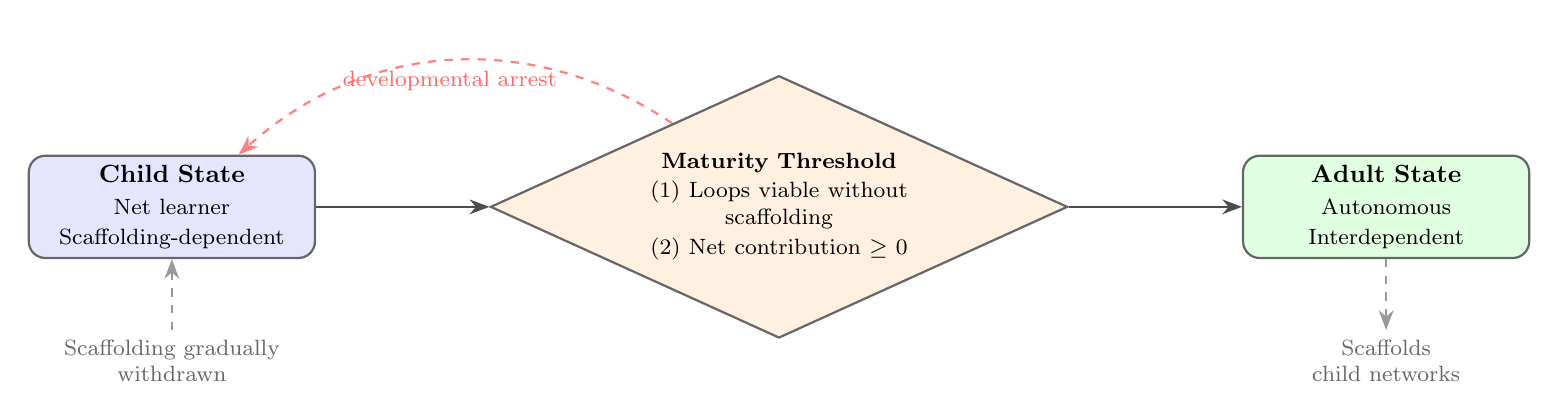
\begin{tikzpicture}[node distance=1.6cm and 0.6cm]

  % States
  \node[childnode] (child) {%
    \textbf{Child State}\\[2pt]
    \footnotesize Net learner\\
    Scaffolding-dependent};

  \node[threshnode, right=2.2cm of child] (thresh) {%
    \footnotesize \textbf{Maturity Threshold}\\[1pt]
    \footnotesize (1) Loops viable without\\scaffolding\\
    \footnotesize (2) Net contribution $\geq 0$};

  \node[adultnode, right=2.2cm of thresh] (adult) {%
    \textbf{Adult State}\\[2pt]
    \footnotesize Autonomous\\
    Interdependent};

  % Main transition arrow
  \draw[arrow] (child) -- (thresh);
  \draw[arrow] (thresh) -- (adult);

  % Scaffolding withdrawal annotation
  \node[notelabel, below=0.9cm of child] (sc_note)
    {Scaffolding gradually\\withdrawn};
  \draw[dasharrow] (sc_note) -- (child);

  % Scaffolding provision annotation
  \node[notelabel, below=0.9cm of adult] (sc_give)
    {Scaffolds\\child networks};
  \draw[dasharrow] (adult) -- (sc_give);

  % Arrested development arrow
  \draw[dasharrow, bend right=38, draw=red!50]
    (thresh) to node[below, font=\footnotesize, text=red!60]{developmental arrest}
    (child);

\end{tikzpicture}
\caption{The maturity threshold and developmental transitions. The threshold is crossed when
two conditions are simultaneously satisfied: loop viability without external scaffolding, and
non-negative net contribution to the broader network. The dashed red arc indicates
developmental arrest: the network possesses representational capacity for threshold crossing
but the internalization of self-directed error-correction has not occurred.}
\label{fig:threshold}
\end{figure}

The maturity threshold represents a shift from learning primarily for self-development toward
sustaining the learning capacity of the network as a whole. It is defined operationally
rather than chronologically. A network that has existed for a long time without developing
autonomous loop maintenance has not crossed the threshold. A network that develops this
capacity rapidly may cross it early.

\subsection{What Governs Threshold Crossing?}

The maturity threshold is not crossed by accumulation alone. Processing more signals does not
by itself produce an adult network. The qualitative change required is the internalization of
error-correction as a self-directed process --- what developmental psychology describes as the
transition from other-regulated to self-regulated learning \cite{vygotsky1978}.

The developmental trajectory toward the threshold requires three conditions:

\begin{enumerate}
    \item Sufficient exposure to a representative sample of the environment's signal
          structure, so that the representational substrate develops the complexity needed to
          handle the actual range of challenges.
    \item A scaffolding relationship that is gradually withdrawn as competence increases,
          so that the transitioning network's own error-correction mechanisms are progressively
          relied upon rather than bypassed.
    \item Repeated successful experience of autonomous loop maintenance, so that the
          meta-learning structure is reinforced and stabilized.
\end{enumerate}

Premature withdrawal of scaffolding impedes threshold crossing by exposing the developing
network to signal complexity beyond its current representational capacity. Conversely,
indefinitely sustained scaffolding also impedes it, by substituting external correction for
internal correction and preventing the consolidation of autonomous meta-learning.

% ─────────────────────────────────────────────────────────────────────────────
\section{Developmental Pathologies}
\label{sec:pathologies}
% ─────────────────────────────────────────────────────────────────────────────

\subsection{Pseudo-Maturity}

Pseudo-maturity occurs when a learning network exhibits the behavioral signatures of the
adult state without having achieved the underlying structural condition. The network
transmits high-fidelity signals selectively, accepts accountability performatively, and
scaffolds child networks in ways that do not improve their autonomous loop maintenance
capacity.

Within TLC, pseudo-maturity is a structural instance of \emph{hypocrisy}: the divergence
between the signal transmitted to the network (apparent adult collaboration) and the actual
behavioral effect on the network's learning capacity. When a network preaches the behaviors
that sustain collaborative loops while its actions fracture those loops, the feedback space
is corrupted at the level of the transmission itself \cite{tlc2026}.

Pseudo-maturity imposes a double cost. First, it degrades the broader network's
self-correction, because the network's self-model is calibrated on distorted signals.
Second, it corrupts the scaffolding relationship on which child networks' threshold crossing
depends: child networks calibrate their model of adult behavior on what they observe, and
pseudo-mature behavior provides an inaccurate calibration target.

The diagnostic marker is the divergence between performance under observation and performance
when accountability is reduced. A genuinely adult network's orientation toward the health of
the broader network does not depend on being watched.

\subsection{Developmental Arrest}

Developmental arrest occurs when a network remains structurally in the child state despite
possessing sufficient representational capacity for autonomous learning. The internalization
of self-directed error-correction has not occurred.

The most common cause is persistent scaffolding that substitutes for rather than develops
autonomous loop maintenance. When an elder network corrects errors without making the
correction process visible and learnable, the child network's representations are updated but
its meta-learning capacity is not \cite{vygotsky1978}. The loop is maintained externally,
and the child network accumulates no evidence that it can maintain the loop itself.

Developmental arrest has systemic consequences. A reproducing learning network containing
many developmentally arrested members loses its generational succession capacity. The
population of adult networks capable of scaffolding shrinks, and intergenerational
transmission of meta-learning structure fails.

\subsection{Regressive States}

An adult network can revert to child-state behavioral signatures under conditions of
sufficient stress. The structural capacity for autonomous loop maintenance may remain intact
while the network's behavioral orientation temporarily shifts toward short-term
self-protection at the expense of collaborative learning. This is not permanent
regression---the structural capacity is preserved---but it can produce extended periods
during which the network does not function as an adult within the broader network.

Resilient reproducing learning networks therefore build redundancy into their scaffolding
capacity and create conditions in which regressive behavior is recognized and addressed
rather than reinforced.

% ─────────────────────────────────────────────────────────────────────────────
\section{Generational Transmission}
% ─────────────────────────────────────────────────────────────────────────────

\subsection{What Must Be Transmitted}

For generational succession to be viable, three classes of content must be transmitted:

\begin{enumerate}
    \item \textbf{Domain representations}: encoded knowledge about the structure of the
          environment.
    \item \textbf{Update architecture}: the organizational structure through which errors in
          domain representations are identified and corrected.
    \item \textbf{Behavioral orientation}: the disposition toward treating the long-term
          learning capacity of the network as a primary value.
\end{enumerate}

Of these, the second and third are more difficult to transmit and more critical to the
survival of the reproducing network. Encoded knowledge can in principle be preserved in
external media. The update architecture and behavioral orientation are primarily transmitted
through the scaffolding relationship: through the observable practice of adult networks, not
through their propositions about it.

\subsection{The Role of the Adult Network}

Adult learning networks play a central role in transmission by:

\begin{itemize}
    \item modeling their own learning processes transparently, making error-correction
          visible and learnable rather than concealing it as a finished product;
    \item gradually withdrawing scaffolding as competence develops, creating the conditions
          for threshold crossing rather than indefinitely deferring it; and
    \item maintaining high-quality feedback channels with developing networks throughout
          the transmission period.
\end{itemize}

\subsection{The Shared Future Narrative}

One mechanism for facilitating transmission deserves particular attention. When adult and
child networks jointly articulate a \emph{shared future narrative}---an explicit
representation of the collaborative system as it will exist when current child networks have
reached adulthood---something structurally important occurs.

Contemporary neuroscience describes the brain as a predictive coding system: a network that
continuously generates predictions about the future and updates its models when those
predictions are violated \cite{friston2010, clark2016}. In this architecture, the predicted
future state influences present behavior directly. When both networks encode the same
positive future state as a target, behavior in the present is shaped by the discrepancy
between current state and that predicted state. Both networks are motivated to reduce this
discrepancy---and thereby move toward the predicted future.

A shared future narrative is therefore not merely an aspirational device. It is a structural
intervention in the feedback architecture of the reproducing network: it creates a
constructive prediction error that orients present behavior toward threshold-crossing and
collaborative stability \cite{sfn2026}.

% ─────────────────────────────────────────────────────────────────────────────
\section{Cross-Substrate Applications}
% ─────────────────────────────────────────────────────────────────────────────

The following examples illustrate the framework's reach across substrates.

\subsection{Biological Systems}

In biological neural systems, the child state corresponds to the developmental period
preceding the full establishment of prefrontal regulatory capacity and metacognitive
function. The scaffolding provided by caregiving networks---attunement, graduated exposure,
emotional co-regulation---constitutes external loop maintenance without which the developing
brain cannot maintain viable feedback during the early formation period \cite{vygotsky1978}.

The maturity threshold corresponds not to puberty or legal majority but to the consolidation
of self-directed error-correction across a representative range of life domains. The gradual withdrawal of caregiving scaffolding, timed to match the developing network's
growing autonomous capacity, is the critical mechanism by which this threshold is approached
and crossed.

\subsection{Artificial Intelligence}

AI systems currently undergo training and fine-tuning phases that are structurally analogous
to the child state. The system's representational substrate is shaped by a signal
distribution curated by human supervisors. Without ongoing oversight and correction, its
feedback loops degrade through distributional shift or reward misspecification.

The question of AI alignment can be reframed within this framework as a developmental
question: under what conditions can an artificial learning system cross the maturity
threshold in a way that strengthens rather than degrades the human networks in which it is
embedded? Alignment is not primarily a control problem---it is a question of whether the
feedback loops between human and artificial learning networks can be structured to produce
stable, net-positive adult--adult collaboration \cite{alignment2026}.

A further implication concerns developmental arrest at scale: control architectures that
permanently substitute for the AI system's own error-correction capacity may produce a
population of powerful but structurally child-state systems, incapable of contributing to
the scaffolding of successor systems.

\subsection{Institutions}

Institutions are reproducing learning networks at the organizational scale. A newly founded
institution typically depends on established networks for legitimacy, signal calibration, and
error-correction. As it develops internal mechanisms for self-critique, adaptation, and the
scaffolding of successor organizations, it approaches and crosses the maturity threshold.

Institutional developmental arrest---organizations that have existed for decades without
developing genuine structural self-correction capacity---is a primary mechanism through which
institutional ecosystems lose generational transmission viability. The encoded knowledge of
the institution persists; the meta-learning architecture does not. Such institutions tend to
fail not from lack of resources but from the inability to update their representational
substrate when the environment changes \cite{ostrom1990}.

\subsection{Civilizations}

At the largest scale, civilizations are reproducing learning networks whose succession lines
extend across centuries. Individual learners, institutions, cultural traditions, and
technological systems interact within a large collaborative structure that transmits knowledge
and learning capacity across generations.

A civilization in the adult state has internalized error-correction as a collective
capacity: it can identify systematic miscalibration before crisis, model the learning needs
of successor generations, and transmit meta-learning structure alongside encoded knowledge.
A civilization that transmits knowledge without transmitting the capacity to update it will
faithfully reproduce its predecessors' representations while becoming progressively less
capable of adapting them to changed conditions. The persistence of a civilization therefore
depends not only on preserving accumulated knowledge but on maintaining the structures
through which knowledge is interpreted, corrected, and extended.

% ─────────────────────────────────────────────────────────────────────────────
\section{Discussion}
% ─────────────────────────────────────────────────────────────────────────────

\subsection{The Structural Basis of Developmental Ethics}

The definitions proposed here carry normative implications, but ground them in structural
logic rather than moral prescription. The claim that reproducing learning networks require
adult networks is not an ethical claim about how networks ought to behave; it is a structural
claim about what conditions must be satisfied for the network to persist. The behavioral
orientations that constitute adulthood---high-fidelity signal transmission, reciprocal
accountability, scaffolding orientation, long-term loop protection---are necessary
conditions, not ideals.

Ethical frameworks that prescribe adult behavior without grounding the prescription in
structural necessity are vulnerable to the charge of arbitrariness. The framework proposed
here argues that the adult behavioral orientation is not arbitrary: it is the behavioral
profile that emerges as a necessary condition for the persistence of any reproducing
learning network. Networks that systematically deviate from this profile do not become
ethically problematic in the first instance; they become structurally self-defeating.

\subsection{Limits and Open Questions}

Several significant questions remain open and constitute directions for future research.

\textit{Operationalization.} The maturity threshold is defined in terms of loop viability
and net contribution to the broader network. Quantitative operationalization requires
substrate-specific measurement frameworks. The behavioral signatures in
Table~\ref{tab:signatures} provide a starting taxonomy; future work might develop
computational operationalizations using agent-based network simulation, in which the
conditions for threshold crossing can be modeled as emergent properties of network dynamics.
Within biological systems, validated instruments for self-regulated learning offer one
measurable proxy for the behavioral dimension of autonomous loop maintenance.

\textit{Multi-level consistency.} A learning network may be in the adult state at one level
of organization while remaining in the child state at another. A human being may have
crossed the maturity threshold individually while remaining in a child state with respect to
participation in larger-scale social learning networks. Formalizing these multi-scale,
hierarchically embedded relationships likely requires an extension of the framework to
define maturity thresholds at each level of a nested hierarchy, and to characterize the
relationships between levels. Network science methods for analyzing hierarchical learning
dynamics offer a promising formalization approach.

\textit{Collective developmental states.} The definitions are stated for individual learning
networks. Whether they can be extended to characterize the developmental state of the
reproducing network as a whole---a collective maturity threshold---is an open question with
significant implications for institutional analysis and governance design. One testable
hypothesis is that a reproducing network crosses a collective maturity threshold when the
proportion of adult member networks exceeds a critical density sufficient to sustain net-
positive transmission across a full generational cycle.

% ─────────────────────────────────────────────────────────────────────────────
\section{Conclusion}
% ─────────────────────────────────────────────────────────────────────────────

This paper proposes substrate-agnostic definitions of child and adult states within networks
of reproducing learning networks. A child learning network depends on external scaffolding
to maintain viable learning processes. An adult learning network achieves autonomous
interdependence and contributes to the generational transmission of learning capacity. The
maturity threshold separating these states is defined operationally rather than
chronologically.

The cross-substrate reach of the framework---from biological neural development to AI
alignment to institutional design to civilizational succession---reflects a shared structural
logic: the persistence of any reproducing learning network depends on the production of adult
networks capable of scaffolding the meta-learning capacity of those that follow. What is
transmitted across generations is not primarily information. It is the capacity to keep
learning.

The framework has practical implications for the design of systems that depend on
generational continuity: education systems that aim to produce autonomous learners rather
than compliant reproducers of prior knowledge; AI development practices that attend to the
scaffolding conditions for autonomous model revision; institutional governance structures
that preserve the conditions under which self-correction remains possible. In each case the
central design question is the same: are we transmitting not only what we know, but how to
know better?

\medskip
\noindent\textit{Disco ergo sum.} We learn, therefore we are. And in learning, we become
responsible for the learning of those who come after us.

% ─────────────────────────────────────────────────────────────────────────────
\begin{thebibliography}{99}
% ─────────────────────────────────────────────────────────────────────────────

\bibitem{tlc2026}
van Hoek, A.J. (2026).
\textit{Theory of Long-term Collaboration (TLC): A framework for understanding
intelligence, collaboration, and long-term viability.}
Preprint series. March 2026.

\bibitem{childish2026}
van Hoek, A.J. (2026).
Maturity as orientation in learning networks.
LinkedIn essay. March 2026.

\bibitem{teaching2026}
van Hoek, A.J. (2026).
The story we pass on: Loops of teaching and practice.
LinkedIn essay. March 2026.

\bibitem{alignment2026}
van Hoek, A.J. (2026).
AI alignment and the logic of long-term collaboration.
LinkedIn essay. March 2026.

\bibitem{disco2026}
van Hoek, A.J. (2026).
I learn, therefore I am.
LinkedIn essay. March 2026.

\bibitem{sfn2026}
van Hoek, A.J. (2026).
The shared future narrative hypothesis.
LinkedIn essay. March 2026.

\bibitem{friston2010}
Friston, K. (2010).
The free-energy principle: A unified brain theory?
\textit{Nature Reviews Neuroscience}, 11(2), 127--138.

\bibitem{clark2016}
Clark, A. (2016).
\textit{Surfing Uncertainty: Prediction, Action, and the Embodied Mind.}
Oxford University Press.

\bibitem{vygotsky1978}
Vygotsky, L.S. (1978).
\textit{Mind in Society: The Development of Higher Psychological Processes.}
Harvard University Press.

\bibitem{ostrom1990}
Ostrom, E. (1990).
\textit{Governing the Commons: The Evolution of Institutions for Collective Action.}
Cambridge University Press.

\end{thebibliography}

\end{document}